\begin{frame}[fragile]
  \partpage

\paragraph{Packages required for reproducing the slides}
\begin{knitrout}
\definecolor{shadecolor}{rgb}{0.969, 0.969, 0.969}\color{fgcolor}\begin{kframe}
\begin{alltt}
\hlkwd{library}\hlstd{(tidyverse)}  \hlcom{# opinionated collection of packages for data manipulation}
\hlkwd{library}\hlstd{(GGally)}     \hlcom{# extension to ggplot vizualization system}
\hlkwd{library}\hlstd{(FactoMineR)} \hlcom{# PCA and oter linear method for dimension reduction}
\hlkwd{library}\hlstd{(factoextra)} \hlcom{# fancy plotting for FactoMineR output}
\hlcom{# color and plots themes}
\hlkwd{library}\hlstd{(RColorBrewer)}
\hlstd{pal} \hlkwb{<-} \hlkwd{brewer.pal}\hlstd{(}\hlnum{10}\hlstd{,} \hlstr{"Set3"}\hlstd{)}
\hlkwd{theme_set}\hlstd{(}\hlkwd{theme_bw}\hlstd{())}
\end{alltt}
\end{kframe}
\end{knitrout}

\end{frame}

\begin{frame}
	\frametitle{Machine Learning}

	\begin{center}
		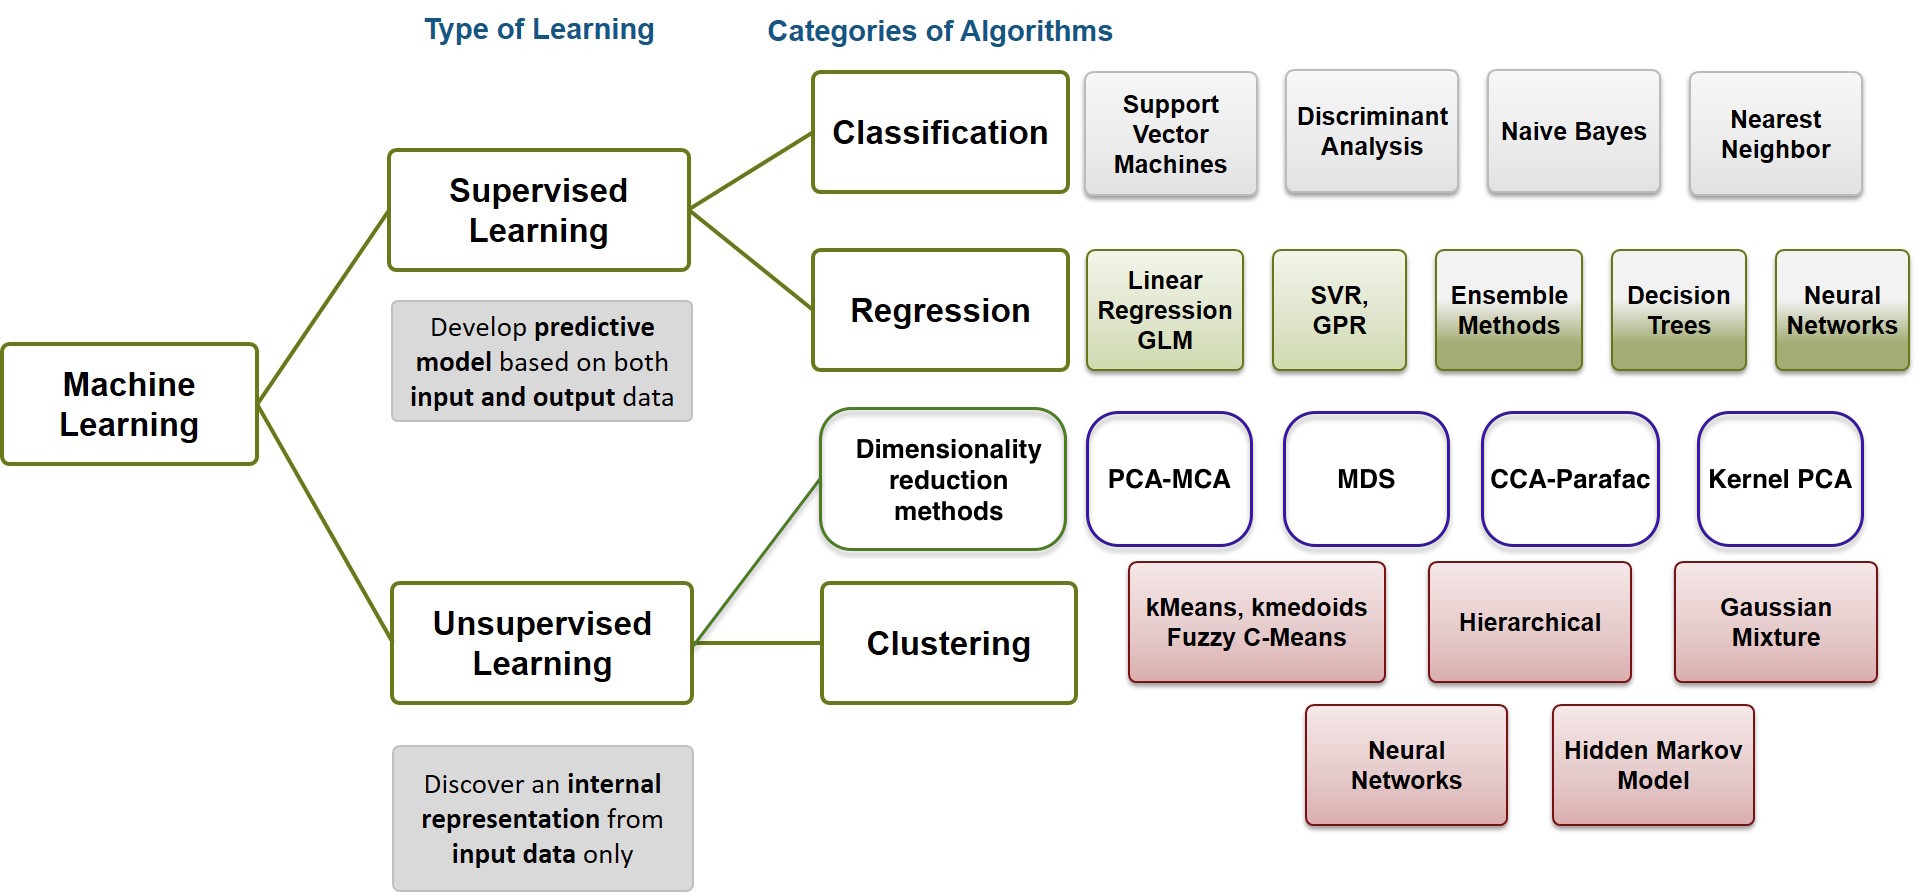
\includegraphics[width=\textwidth]{Learning+Types}
	\end{center}

\end{frame}

\begin{frame}
  \frametitle{Supervised vs Unsupervised Learning}

  \begin{block}{Supervised Learning}
    \begin{itemize}
    \item Training data $\mathcal{D}_n = \{(\bx_1, y_1), \ldots, (\bx_n, y_n)\}, X_i \sim^{\text{i.i.d}} \mathbb{P}$
    \item Construct a predictor $\hat f : \mathcal{X} \rightarrow \mathcal{Y}$ using $\mathcal{D}_n$
    \item Loss $\ell(y, f(x))$ measures how well $f(x)$ predicts $y$
    \item Aim: minimize the generalization error
    \item Task: Regression, Classification
    \end{itemize}
    $\rightsquigarrow$ The goal is clear: predict $y$ based on $x$ (regression, classification)
  \end{block}

  \begin{block}{Unsupervised Learning}
  \begin{itemize}
    \item Training data $\mathcal{D} = \{\bx_1, \ldots, \bx_n\}$
    \item Loss? , Aim?
    \item Task: \alert{\bf Dimension reduction}, Clustering
  \end{itemize}
  $\rightsquigarrow$ The goal is less well defined, and \emph{validation} is questionable
  \end{block}

\end{frame}

\begin{frame}
\frametitle{Dimension Reduction?}

\begin{figure}
  \includegraphics<1>[height=.5\textheight]{belardi-camel-3d-4}
  \includegraphics<2>[height=.5\textheight]{belardi-camel-3d-3}
  \includegraphics<3>[height=.5\textheight]{belardi-camel-3d-2}
  \caption{\tiny source: F. Belardi}
\end{figure}

\begin{itemize}
\item How to view a high-dimensional dataset ?
\item High-dimension: dimension larger than 2!
\item \emph{Projection} in a 2D space.
\end{itemize}
\end{frame}

\begin{frame}[fragile]
  \frametitle{Companion data set: 'crabs'}
  \framesubtitle{Morphological Measurements on Leptograpsus Crabs}

\begin{block}{Description: \textcolor{black}{\it small data, low-dimensional}}
\small The crabs data frame has 200 rows and 8 columns, describing 5 morphological measurements on 50 crabs each of two colour forms and both sexes, of the species \textit{Leptograpsus variegatus} collected at Fremantle, W. Australia.\\
\end{block}

\begin{figure}
  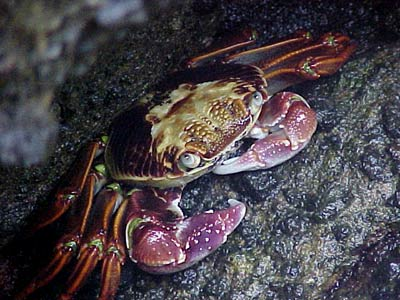
\includegraphics[width=3cm]{crab}
  \caption{A leptograpsus Crab}
\end{figure}
\end{frame}

\begin{frame}[fragile,allowframebreaks]
  \frametitle{Companion data set: 'crabs'}
  \framesubtitle{Table header}

\begin{knitrout}
\definecolor{shadecolor}{rgb}{0.969, 0.969, 0.969}\color{fgcolor}\begin{kframe}
\begin{alltt}
\hlstd{crabs} \hlkwb{<-} \hlstd{MASS}\hlopt{::}\hlstd{crabs} \hlopt \hlkwd{select}\hlstd{(}\hlopt{-}\hlstd{index)} \hlopt
  \hlkwd{rename}\hlstd{(}\hlkwc{sex} \hlstd{= sex,}
         \hlkwc{species}         \hlstd{= sp,}
         \hlkwc{frontal_lob}     \hlstd{= FL,}
         \hlkwc{rear_width}      \hlstd{= RW,}
         \hlkwc{carapace_length} \hlstd{= CL,}
         \hlkwc{carapace_width}  \hlstd{= CW,}
         \hlkwc{body_depth}      \hlstd{= BD)}
\hlstd{crabs} \hlopt \hlkwd{select}\hlstd{(sex, species)} \hlopt \hlkwd{summary}\hlstd{()} \hlopt \hlstd{knitr}\hlopt{::}\hlkwd{kable}\hlstd{(}\hlstr{"latex"}\hlstd{)}
\end{alltt}
\end{kframe}
\begin{tabular}{l|l|l}
\hline
  & sex & species\\
\hline
 & F:100 & B:100\\
\hline
 & M:100 & O:100\\
\hline
\end{tabular}

\begin{kframe}\begin{alltt}
\hlkwd{dim}\hlstd{(crabs)}
\end{alltt}
\begin{verbatim}
## [1] 200   7
\end{verbatim}
\end{kframe}
\end{knitrout}

\begin{knitrout}
\definecolor{shadecolor}{rgb}{0.969, 0.969, 0.969}\color{fgcolor}\begin{kframe}
\begin{alltt}
\hlstd{crabs} \hlopt \hlkwd{head}\hlstd{(}\hlnum{15}\hlstd{)} \hlopt \hlstd{knitr}\hlopt{::}\hlkwd{kable}\hlstd{(}\hlstr{"latex"}\hlstd{)}
\end{alltt}
\end{kframe}
\begin{tabular}{l|l|r|r|r|r|r}
\hline
species & sex & frontal\_lob & rear\_width & carapace\_length & carapace\_width & body\_depth\\
\hline
B & M & 8.1 & 6.7 & 16.1 & 19.0 & 7.0\\
\hline
B & M & 8.8 & 7.7 & 18.1 & 20.8 & 7.4\\
\hline
B & M & 9.2 & 7.8 & 19.0 & 22.4 & 7.7\\
\hline
B & M & 9.6 & 7.9 & 20.1 & 23.1 & 8.2\\
\hline
B & M & 9.8 & 8.0 & 20.3 & 23.0 & 8.2\\
\hline
B & M & 10.8 & 9.0 & 23.0 & 26.5 & 9.8\\
\hline
B & M & 11.1 & 9.9 & 23.8 & 27.1 & 9.8\\
\hline
B & M & 11.6 & 9.1 & 24.5 & 28.4 & 10.4\\
\hline
B & M & 11.8 & 9.6 & 24.2 & 27.8 & 9.7\\
\hline
B & M & 11.8 & 10.5 & 25.2 & 29.3 & 10.3\\
\hline
B & M & 12.2 & 10.8 & 27.3 & 31.6 & 10.9\\
\hline
B & M & 12.3 & 11.0 & 26.8 & 31.5 & 11.4\\
\hline
B & M & 12.6 & 10.0 & 27.7 & 31.7 & 11.4\\
\hline
B & M & 12.8 & 10.2 & 27.2 & 31.8 & 10.9\\
\hline
B & M & 12.8 & 10.9 & 27.4 & 31.5 & 11.0\\
\hline
\end{tabular}


\end{knitrout}
\end{frame}

\begin{frame}[fragile]
  \frametitle{Companion data set: 'crabs'}
  \framesubtitle{Pairs plot of attributes}

\begin{knitrout}
\definecolor{shadecolor}{rgb}{0.969, 0.969, 0.969}\color{fgcolor}\begin{kframe}
\begin{alltt}
\hlkwd{ggpairs}\hlstd{(crabs,} \hlkwc{columns} \hlstd{=} \hlnum{3}\hlopt{:}\hlnum{7}\hlstd{,} \hlkwd{aes}\hlstd{(}\hlkwc{colour} \hlstd{= species,} \hlkwc{shape} \hlstd{= sex))}
\end{alltt}
\end{kframe}
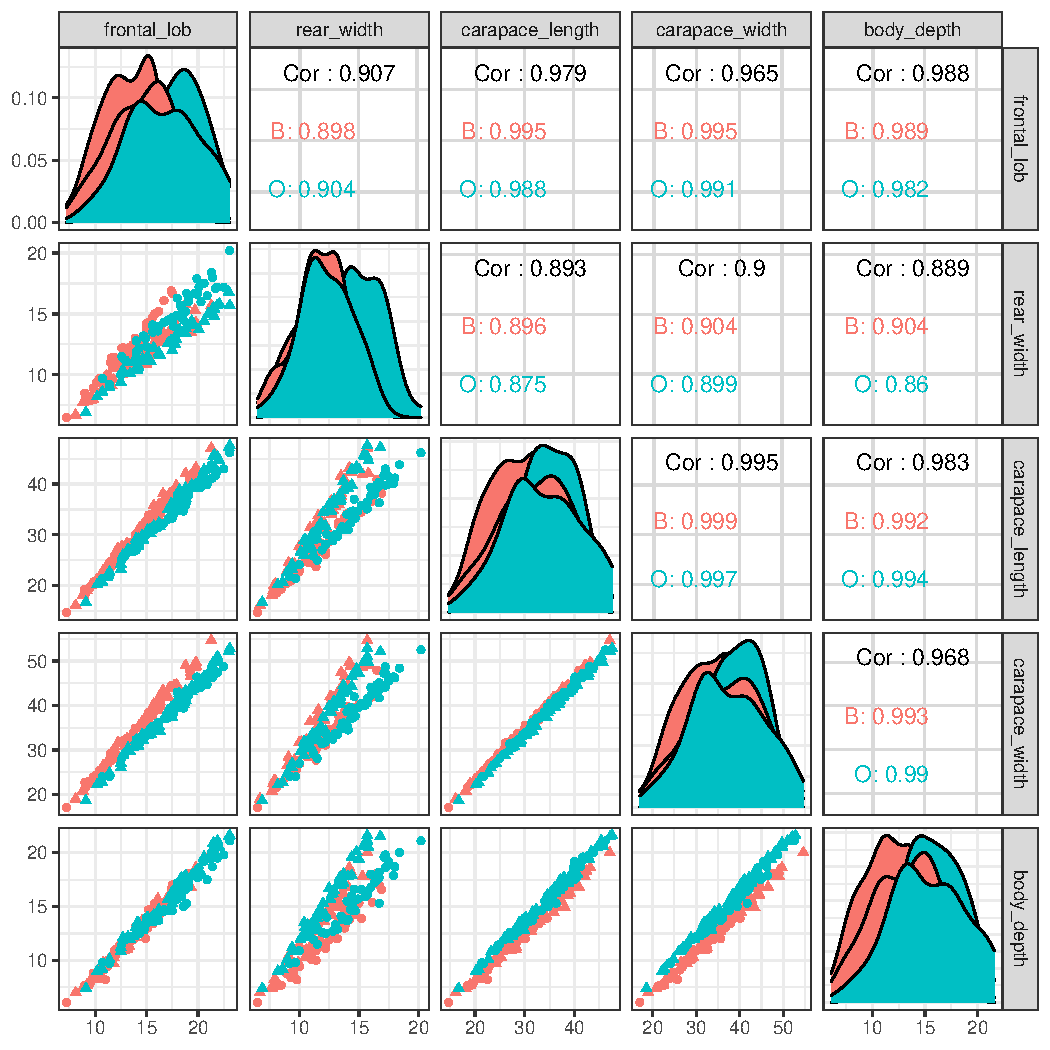
\includegraphics[width=\maxwidth]{figure/crabs_attributes-1} 

\end{knitrout}
$\rightsquigarrow$ Pairs plot don't help...
\end{frame}

\begin{frame}[fragile]
  \frametitle{Companion data set: 'crabs'}
  \framesubtitle{Correlation matrix}

\begin{knitrout}
\definecolor{shadecolor}{rgb}{0.969, 0.969, 0.969}\color{fgcolor}\begin{kframe}
\begin{alltt}
\hlstd{crabs} \hlopt  \hlkwd{select}\hlstd{(}\hlopt{-}\hlstd{species,} \hlopt{-}\hlstd{sex)} \hlopt \hlkwd{cor}\hlstd{( )} \hlopt \hlkwd{kable}\hlstd{(}\hlstr{'latex'}\hlstd{,} \hlkwc{digits} \hlstd{=} \hlnum{3}\hlstd{)}
\end{alltt}
\end{kframe}
\begin{tabular}{l|r|r|r|r|r}
\hline
  & frontal\_lob & rear\_width & carapace\_length & carapace\_width & body\_depth\\
\hline
frontal\_lob & 1.000 & 0.907 & 0.979 & 0.965 & 0.988\\
\hline
rear\_width & 0.907 & 1.000 & 0.893 & 0.900 & 0.889\\
\hline
carapace\_length & 0.979 & 0.893 & 1.000 & 0.995 & 0.983\\
\hline
carapace\_width & 0.965 & 0.900 & 0.995 & 1.000 & 0.968\\
\hline
body\_depth & 0.988 & 0.889 & 0.983 & 0.968 & 1.000\\
\hline
\end{tabular}


\end{knitrout}

\bigskip

\alert{Very high correlation!}
\begin{itemize}
 \item much redundancy?
 \item hidden factor?
\end{itemize}
$\rightsquigarrow$ dimension reduction might hem
\end{frame}

\begin{frame}[fragile]
  \frametitle{Another example: 'snp'}
  \framesubtitle{Genetics variant in European population}

\begin{block}{Description: \textcolor{black}{\it medium/large data, high-dimensional}}
500, 000 Genetics variants (SNP -- Single Nucleotide Polymorphism) for  3000 individuals
(1 meter $\times$ 166 meter (height $\times$ width)
\end{block}

\begin{multicols}{2}
  \begin{itemize}
  \item SNP : 90 \% of human genetic variations
  \item coded as 0, 1 or 2 (10, 1 or 2 allel different against the population reference)
  \end{itemize}

  \begin{figure}
    \centering
     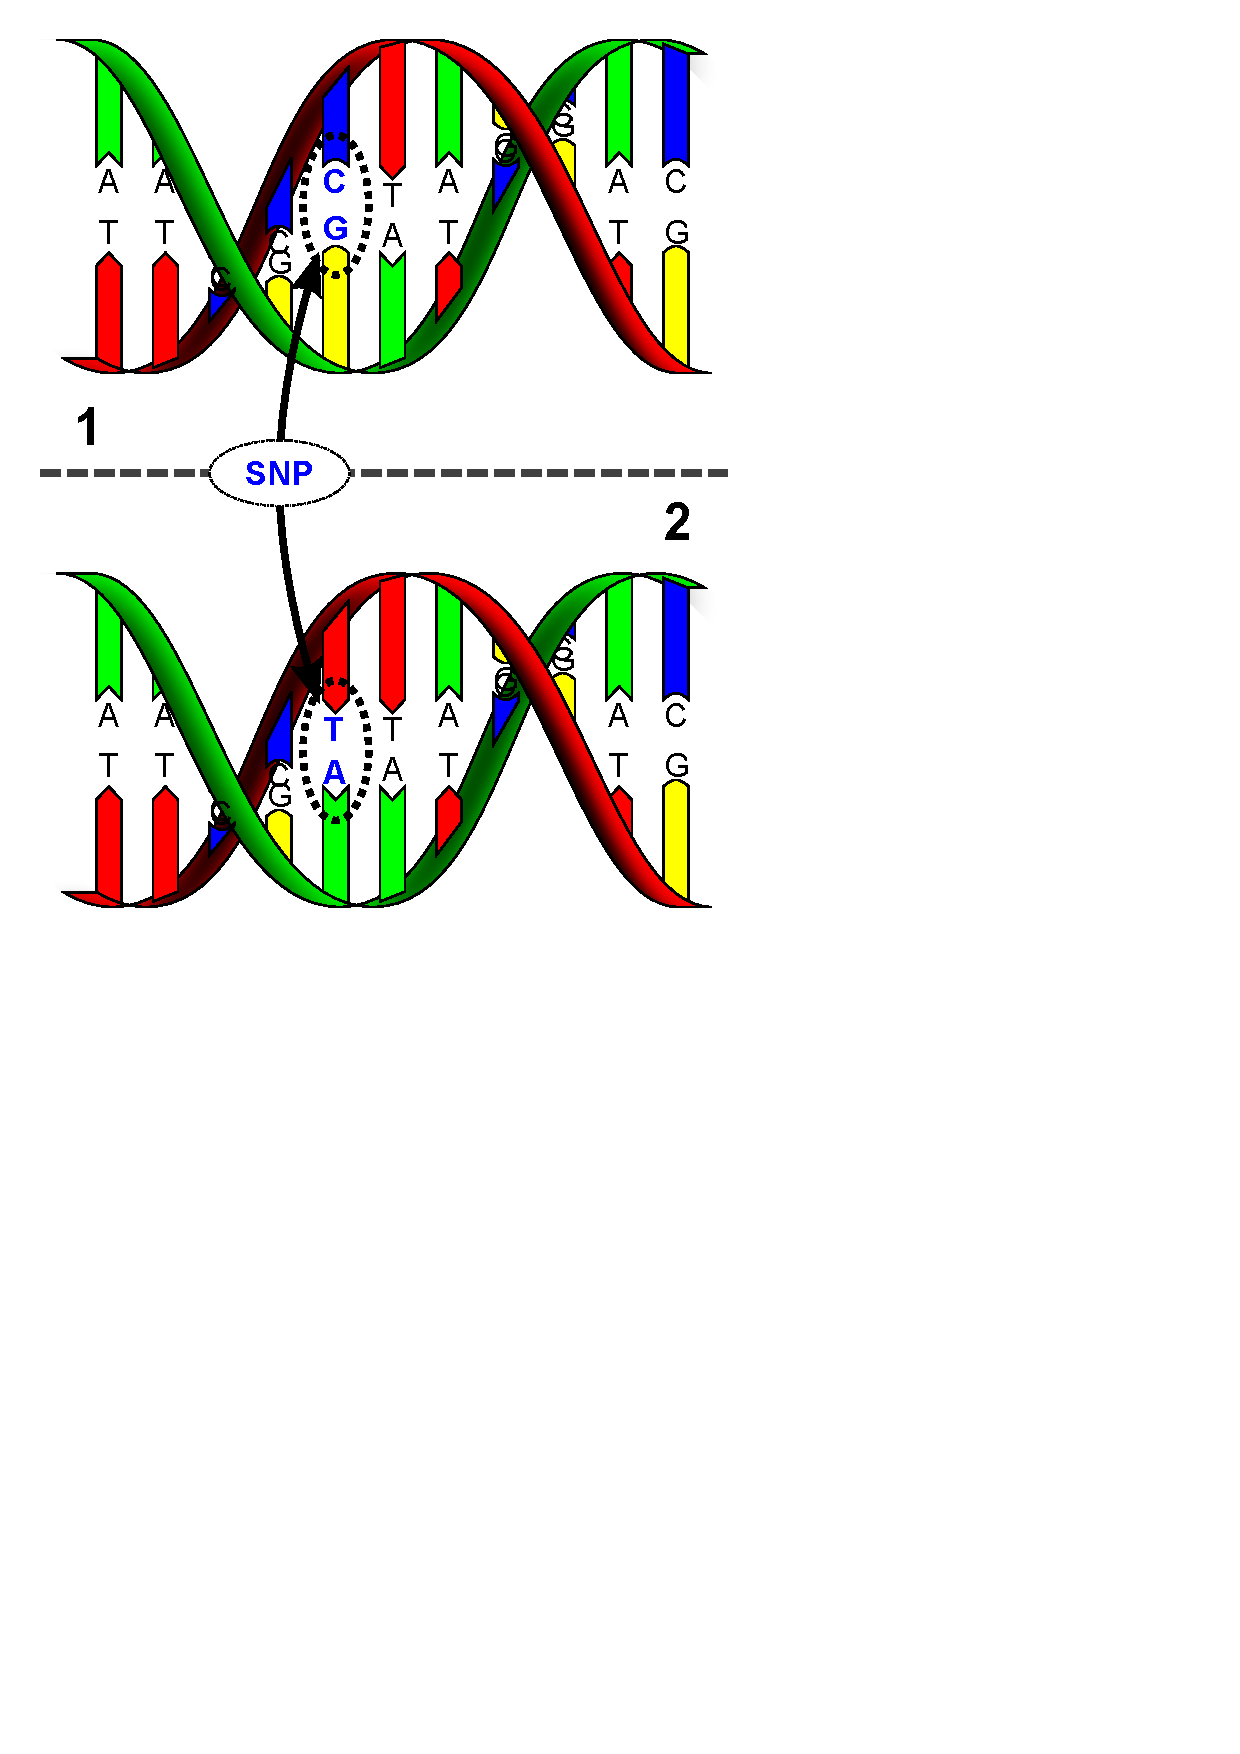
\includegraphics[height=4cm]{SNP}   
    \caption{SNP (wikipedia)}
  \end{figure}
\end{multicols}

\end{frame}

\begin{frame}
  \frametitle{Summarize 500,000 variables in 2}

  \begin{figure}
    \centering
      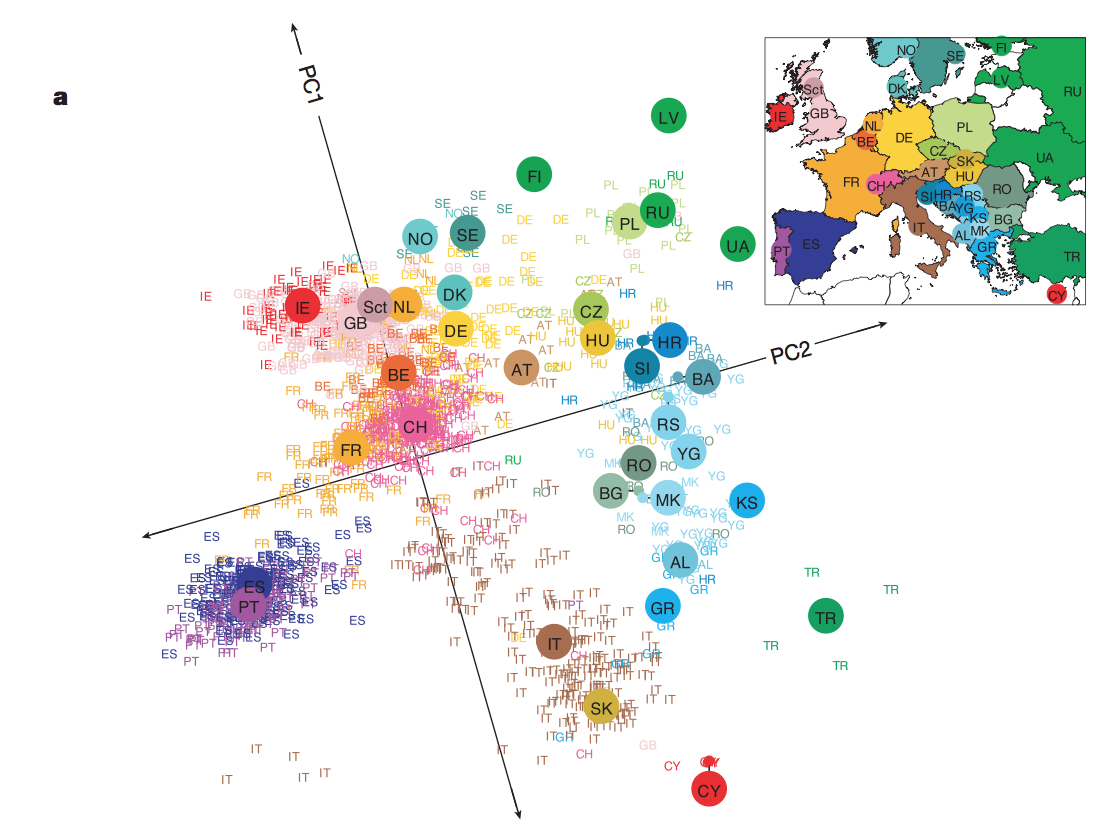
\includegraphics[height=6cm]{geneMirrorGeography}
    \caption{PCA output {\tiny source: Nature "Gene  Mirror Geography Within  Europe", 2008}}
  \end{figure}

  $\rightsquigarrow$ How much information is lost?

\end{frame}


\begin{frame}
\frametitle{Theoretical argument: dimensionality Curse}

\begin{block}{High Dimension Geometry Curse}
\begin{itemize}
\item Folks theorem: In high dimension, everyone is alone.
\item Theorem: If $\bx_1,\ldots, \bx_n$ in the
hypercube of dimension $d$  such
that their coordinates are i.i.d then
\begin{align*}
\mspace{-20mu} d^{-1/p} \left( \max \|\bx_i-\bx_{i'}\|_p - \min \|\bx_i-\bx_{i'}\|_p
\right)  &= 0 + O\left(\sqrt{\frac{\log n}{d}}\right)\\
\frac{\max \|\bx_i-\bx_{i'}\|_p}{\min \|\bx_i-\bx_{i'}\|_p} &= 1 +
O\left(\sqrt{\frac{\log n}{d}}\right).
\end{align*}
\end{itemize}
\end{block}

  $\rightsquigarrow$ When $d$ is large, all the points are almost equidistant\\

  Hopefully, the data \alert{\bf are not really leaving in $d$} dimension (think of the SNP example)

\end{frame}

\begin{frame}
  \frametitle{Dimension reduction: goals summary}

  \paragraph{Main objective:} find a \alert{\bf low-dimensional representation} that captures the "essence" of (high-dimensional) data

  \vfill

  \begin{block}{Application in Machine Learning}
  Preprocessing, Regularization
  \begin{itemize}
    \item compression, denoising,  anomaly detection
    \item Reduce overfitting in supervised learning (improve performances)
  \end{itemize}
  \end{block}

\vfill

  \begin{block}{Application in statistics and data analysis}
    Better understand the data 
    \begin{itemize}
      \item descriptive/exploratory methods
      \item visualization: difficult to plot and interpret $> 3d$!
    \end{itemize}
  \end{block}

\end{frame}

\begin{frame}
  \frametitle{Dimension reduction: problem setup}

    \begin{block}{Settings}
      \begin{itemize}
        \item \alert{Training data } : $\mathcal{D}=\{\bx_1,\ldots,\bx_n\} \in \Rset^d$,   (i.i.d.)
        \item Space $\Rset^d$ of possibly high dimension $(n \ll d)$
      \end{itemize}
    \end{block}

    \vfill
    
    \begin{block}{Dimension Reduction Map}
       Construct a map $\Phi$ from the space $\Rset^{d}$ into a space $\Rset^{d'}$ of \alert{smaller dimension}:
      \begin{align*}
          \Phi:\quad & \Rset^d \to \Rset^{d'}, d' \ll d\\
                     & \bx \mapsto \Phi(\bx)
      \end{align*}
    \end{block}
    
\end{frame}
 
\begin{frame}
  \frametitle{How should we design/construct $\Phi$?}

  \paragraph{Criterion}
  \begin{itemize}
    \item \alert{\bf Geometrical approach}
    \item Reconstruction error
    \item Relationship preservation
  \end{itemize}

  \vfill
  
  \paragraph{Form of the map $\Phi$}
  \begin{itemize}
    \item \alert{\bf Linear} or non-linear ?
    \item tradeoff between \alert{\bf interpretability} and versatility ?
    \item tradeoff between high or \alert{\bf low} computational resource
  \end{itemize}

\end{frame}
